\section{Network Analysis}
As previously mentioned, the friendship network of Yelp is rather incomplete: the majority of users does not have any connections. The users that participate on the social network, however, are highly connected, since $40.92$\% of them are in the large connected component, which means that only $1.80$\% of the OSN participants are absent. The average degree of the whole network is $4.68$ and the clustering coefficient is $0.06$.

Yelp provides an option for users to vote in reviews that they found useful. Figure~\ref{fig:clo_use} relates the closeness centrality to the total useful votes received by a user. We observe that there are roughly three situations: users with low centrality and low usefulness; users with high centrality and low usefulness; and users with high centrality and high usefulness. There is not such a configuration in which users with high usefulness have low centrality. This is a motivation to consider the network structure as an evidence for profile of reviewers.

\begin{figure}[H]
\centering
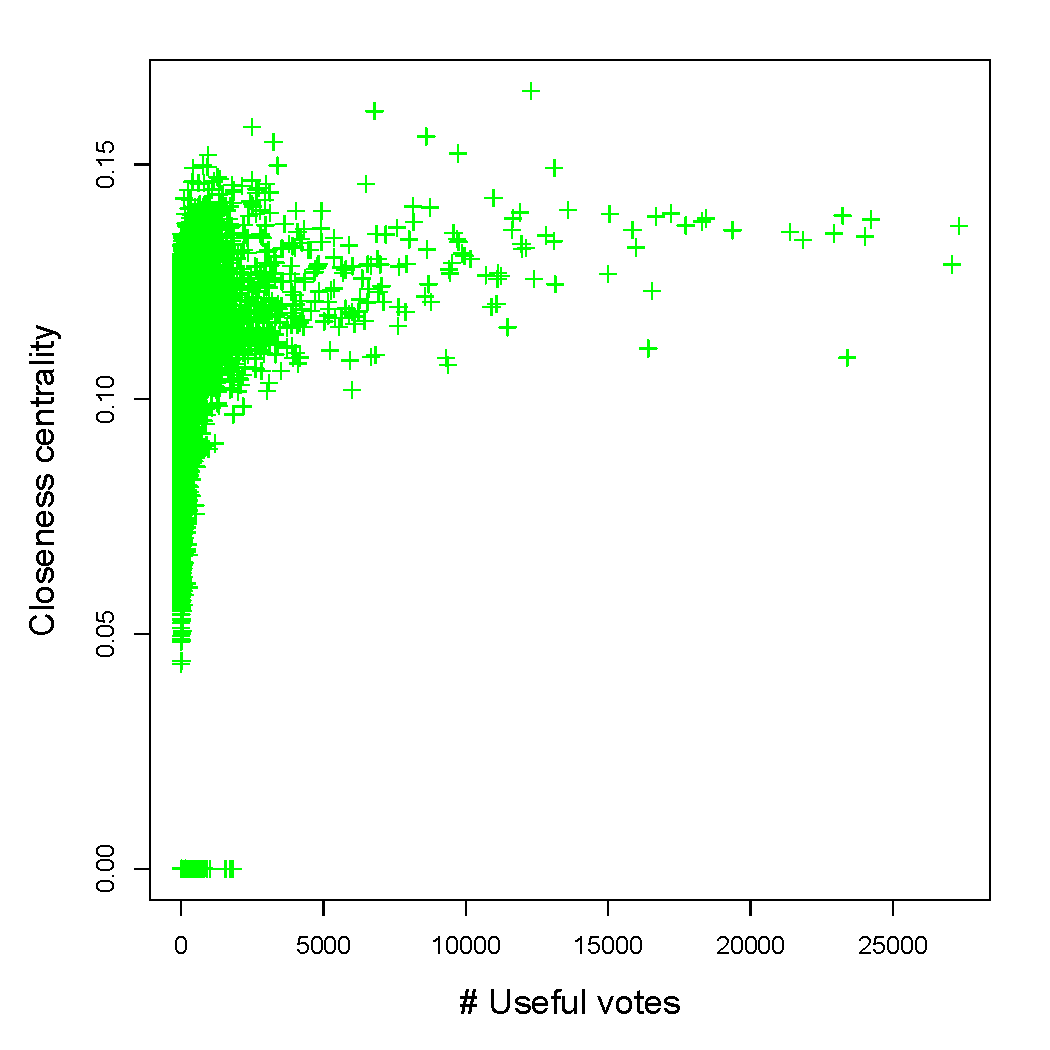
\includegraphics[scale=0.5]{img/close_useful_scatter}
\caption{Correlation between closeness centrality and the number of useful votes for a reviewer.}
\label{fig:clo_use}
\end{figure}

The third set of users cited, a minority, corresponds to reviewers that influence a lot of people. However, few useful votes might indicate that those reviewers provide important experiences for only certain kind of people. Thus, it is necessary to investigate further those reviewers in order to present the information they provide to the ones interested.

\subsection{Homophilly Investigation}

Aiming to validate the presence of homophilly in the network, it was conducted the following experiment: for each edge on the network, the business overlap was computed considering the jaccard similarity of reviewed establishments; a similar process was perfomed for a modified graph with the same nodes and number of edges, which were randomly assigned to pairs. The empirical cumulative distribution of the overlap values are depicted on figure \ref{fig:bus_olap}. We observe a clear difference between the real and the random graphs --- the second practically do not contain positive overlaps, while the first present some.

\begin{figure}[H]
\centering
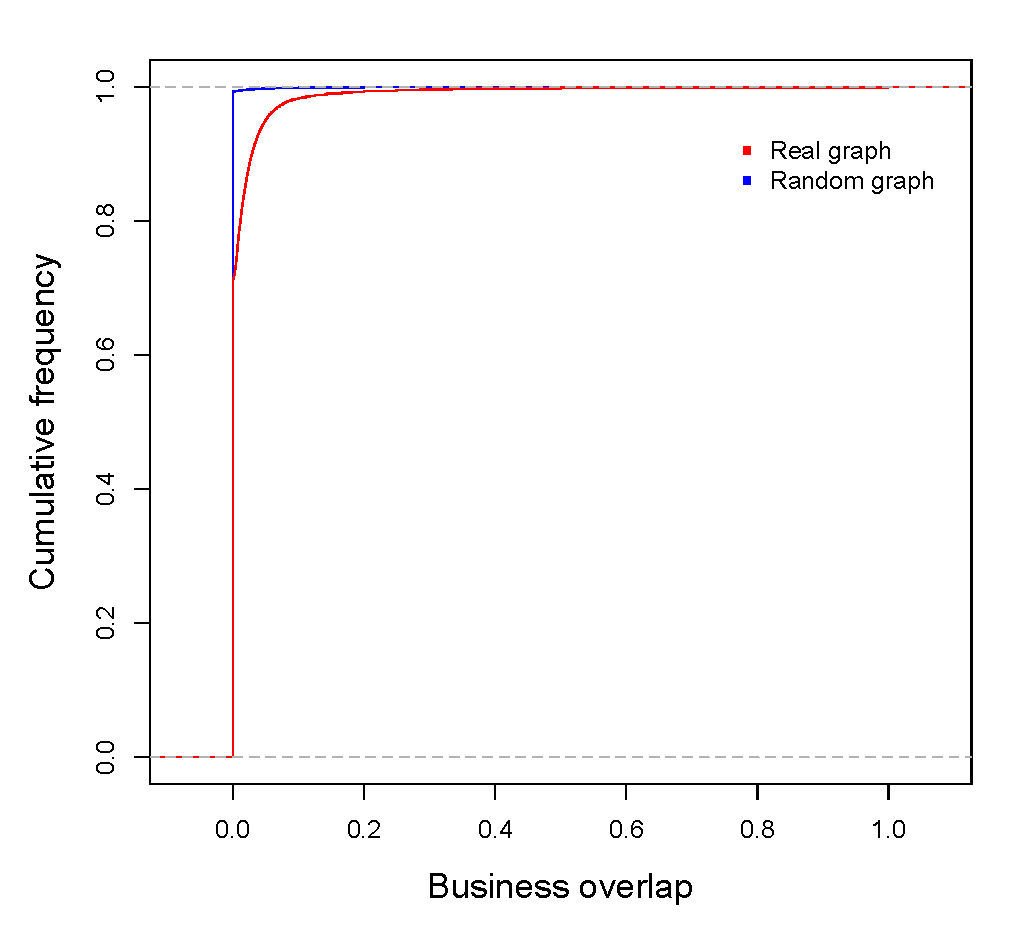
\includegraphics[scale=0.5]{img/ecdf_bus_olap}
\caption{Empirial cumulative distribution of business overlap on real and random graphs.}
\label{fig:bus_olap}
\end{figure}

